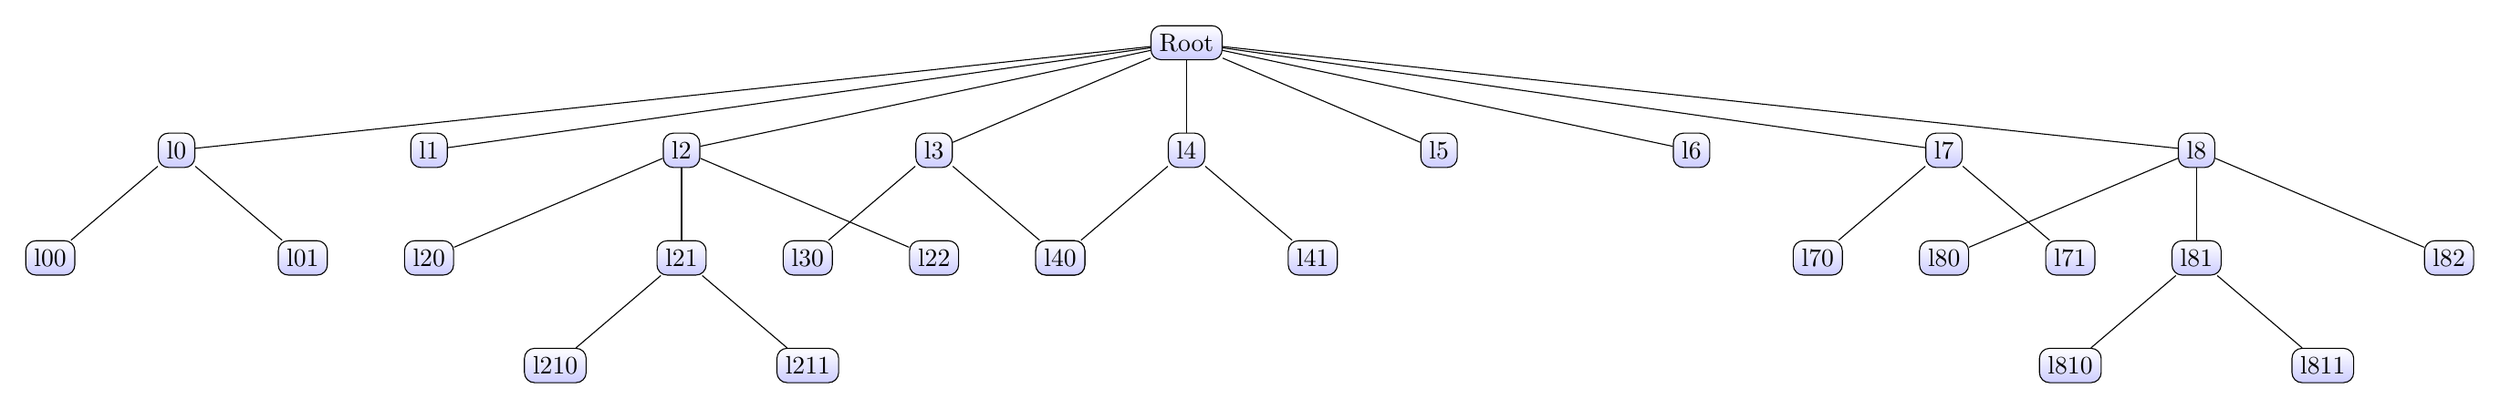
\begin{tikzpicture}[sibling distance=10em, every node/.style = {shape=rectangle, rounded corners, draw, align=center,top color=white, bottom color=blue!20}]]\node {Root}
	child { node {l0} 
		child { node {l00} }		child { node {l01} }}	child { node {l1} }	child { node {l2} 
		child { node {l20} }		child { node {l21} 
			child { node {l210} }			child { node {l211} }}		child { node {l22} }}	child { node {l3} 
		child { node {l30} }		child { node {l31} }}	child { node {l4} 
		child { node {l40} }		child { node {l41} }}	child { node {l5} }	child { node {l6} }	child { node {l7} 
		child { node {l70} }		child { node {l71} }}	child { node {l8} 
		child { node {l80} }		child { node {l81} 
			child { node {l810} }			child { node {l811} 
}}		child { node {l82} }};
\end{tikzpicture}